\chapter{De la criptografía clásica a la de clave pública}

A lo largo de la historia tuvieron lugar una serie de avances que propiciaron la aparición de la criptografía de clave pública. 


En 1917 \textbf{Gilbert Sandford Vernam} (1890-7 de febrero de 1960) inventó un cifrado en flujo y más tarde coinventó un cifrado de libreta de un solo uso. Vernam propuso un teletipo cifrado en el cual una clave previamente preparada y almacenada en cinta perforada se combina carácter por carácter con el mensaje en texto plano para obtener un texto cifrado. Para descifrar el texto cifrado, debe combinarse de nuevo con la clave carácter a carácter para producir el mensaje en texto plano.

Poco tiempo después, \textbf{Joseph Mauborgne}, en aquel entonces capitán en el US Army Signal Corps, propuso, además, que la cinta de papel con la llave tuviera información aleatoria. 

Las dos ideas, cuando se combinan, implementan de manera automática una \textbf{libreta de un solo uso}, aunque ninguno de los dos inventores usó este nombre.

Aunque estos pequeños avances puedan parecer muy antiguos y lejanos, lo cierto es que están muy presentes en nuestro día a día. Por ejemplo, el cifrado de flujo sigue siendo utilizado\footnote{Se emplea una adaptación del mismo} en los teléfonos móviles.

\begin{center}
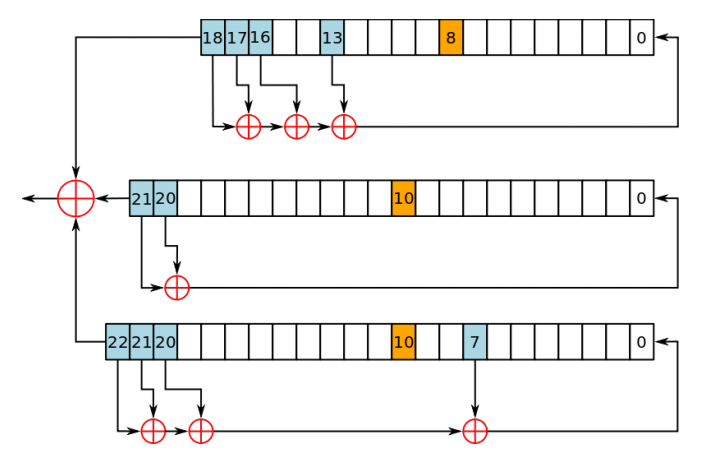
\includegraphics[width=0.6\textwidth]{img/cifrado_flujo.png}
\end{center}

\section{Enigma}
La máquina \textbf{enigma} funcionaba de acuerdo al siguiente esquema:
\begin{center}
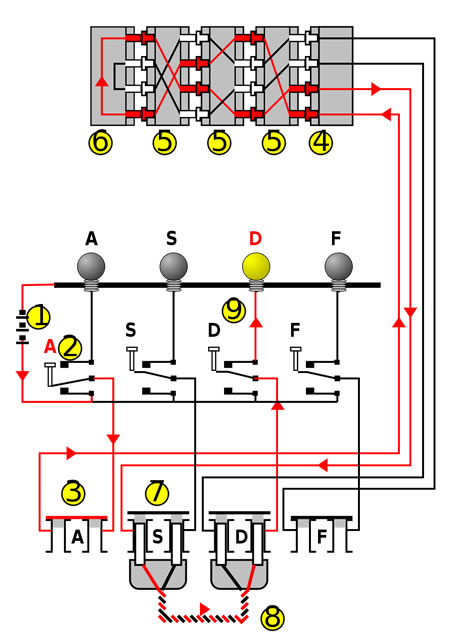
\includegraphics[width=0.6\textwidth]{img/enigma.jpg}
\end{center}
donde el número 8 representa uno de los modificadores, que simplemente conectaba pares de letras para que fuesen intercambiadas; el número 5 representa los rotores y el número 6 el reflector.

En rojo podemos ver el flujo que seguiría la corriente en caso de que pulsásemos la letra $A$, que sería cifrada a una $D$.

\obs La configuración que se muestra en la imagen sólo se mantendría fija durante un brevísimo periodo de tiempo. Tras finalizar el cifrado de la letra $A$, los rotores girarían de modo que no se volvería a seguir el mismo camino nunca más.

Si tenemos una máquina de enigma que funcione con 26 letras, 5 rotores de entre los que hay que escoger 3 y modificando 6 pares de letras\footnote{Es decir, tenemos 6 modificadores}, la pregunta que surge es clara, ¿Cuántas claves posibles tenemos?

Para empezar tenemos que escoger qué tres rotores tomamos, teniendo en cuenta que importa el orden, con lo que tenemos $5\cdot 4 \cdot 3 = 60$ opciones posibles.

Una vez hemos escogido los rotores, debemos ver qué posición tendrá cada rotor. Puesto que tenemos 26 posiciones para cada rotor tenemos un total de $26^3$ opciones.

Por último debemos colocar los modificadores, para lo que tenemos que elegir 6 pares de letras. Para ello tenemos un total de
\[{26 \choose 2} \cdot {24\choose 2}\cdot {22\choose 2}\cdot {20\choose 2}\cdot {18\choose 2}\cdot {16\choose 2} \text{ opciones }\]

Pero, puesto que no importa el orden, debemos dividir entre $6!$.

Agrupando todo lo que hemos mencionado, tenemos que la máquina \textbf{enigma} permite tener un total de:
\[\frac{60\cdot 26^3 \cdot {26 \choose 2} \cdot {24\choose 2}\cdot {22\choose 2}\cdot {20\choose 2}\cdot {18\choose 2}\cdot {16\choose 2}}{6!}\approx 8.469 \cdot 10^{17}  \text{ claves }\]

La forma de trabajar con \textbf{enigma} era mediante un libro de claves donde cada clave era empleada a lo largo de todo el día para todas las comunicaciones.

No obstante, si toda la flota empleaba el mismo sistema de cifrado y los mensajes eran fácilmente interceptables (se comunicaban por radio) al final sería relativamente sencillo que el enemigo descifrara la clave. Para solucionar esto, lo que se hacía es que al comienzo de cada mensaje se enviaban 3 letras, que indicaban la nueva posición de los rotores que debería emplearse a partir de ese momento.

Así, un esquema de transmisión del mensaje sería:
\begin{enumerate}
\item Montamos la máquina con la clave del día.
\item Transmitimos la clave del mensaje dos veces.
\item Cambiamos la posición de los rotores según la clave que enviamos.
\item Transmitimos el mensaje.
\end{enumerate}

Aquí tenemos la debilidad del criptosistema, el envío de la clave dos veces, puesto que nos adelanta cierta información acerca de la posición inicial de los rotores. Otro problema radicó en el hecho de que el primer mensaje del día siempre informaba del tiempo y siempre comenzaba de la misma forma, lo que daba aún más información al bando rival.

A la hora de descifrar, el mecanismo es sencillo. La forma en que funciona \textbf{enigma} está basada en trasposiciones. Es decir, si a partir de la letra $A$ obtengo la $B$, a partir de la $B$ obtendré la $A$, partiendo de la misma clave.

Por tanto, una vez recibido el mensaje lo único que hay que hacer es introducir el mensaje cifrado en la máquina y como salida obtendremos el texto original.

Veamos por qué esto es cierto:
\begin{proof}
Para comprobar que la función de cifrado y su inversa son la misma, vamos a ver cómo funcionaba \textbf{enigma} sobre cada letra.

En primer lugar se intercambiaba una letra por otra mediante los modificadores. Tras esto la letra pasa por los rotores y llega al reflector (que será la clave de la demostración) y tras ello vuelve a pasar por los rotores y por el modificador.

Así nos queda que
\[\rho(m) = σ^{-1}δ^{1}Rδσ(m) \implies \rho^{-1}(m) = σ^{-1}δ^{1}Rδσ(m) = \rho(m)\]
\end{proof}

Pero ahora el lector avispado se percatará de un detalle muy importante. De todas las claves posibles que mencionamos al inicio de esta sección, no todas darán lugar a una función $\rho$ que coincida con su inversa.

En este caso, $\rho = \rho^{-1} \iff \rho = (a_1a_2)(a_3a_4)...(a_{25}a_{26})$, puesto que necesitamos que $\rho$ no haga más que permutar pares de letras.

Dada esta restricción tendremos un total de
\[\frac{{26 \choose 2} {24 \choose 2} ... {2 \choose 2}}{13!} =\frac{26!}{13!2^{13}} \approx 1.01 \cdot 10^{15} \text{ claves posibles }\]

\section{Criptosistemas de clave simétrica}
Todos los sistemas que hemos visto hasta ahora, englobados como criptosistemas clásicos, comparten una misma propiedad: \textit{Si sabemos cómo cifrar sabremos cómo descifrar}. Esto se debe a que todos estos sistemas son de \textbf{clave simétrica}.

Si pretendemos que diferentes usuarios puedan emplear el mismo criptosistema manteniendo seguridad entre ellos, necesitaremos una clave distinta para cada uno de ellos.

En el mundo de la tecnología en que vivimos ahora mismo esto es inviable puesto que serían necesarias demasiadas claves (una por usuario/actividad). Además, al llegar un nuevo usuario sería necesario compartir con él la clave de alguna forma.

La solución se encuentra en las \textbf{funciones de un solo sentido} como $f(n)=3^{n}$ en $\mathbb{F}_{1231}^*$:
\begin{center}
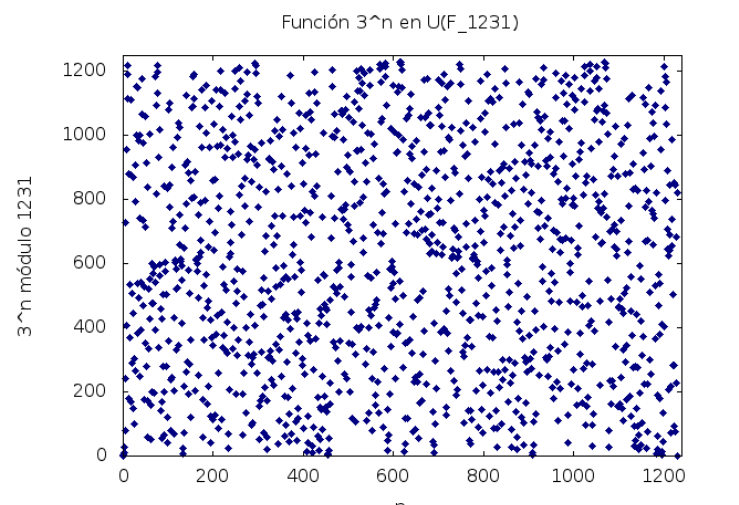
\includegraphics[width=0.7\textwidth]{img/3nF1231.png}
\end{center}

\newpage

\begin{defn}[Función de un sólo sentido]
Sea $\appl{f}{A}{B}$ una función inyectiva, se dice que es \textbf{de un sólo sentido} si:
\begin{enumerate}
\item $f(a)$ es fácil de calcular
\item Dado $b \in Im(f)$ podemos encontrar $a\tq f(a) = b$ pero, en la práctica, es difícil de encontrar.
\end{enumerate}
\end{defn}

Como ejemplo trivial podemos considerar un puzle y la función $f$ que consiste en desmontarlo. Esta función es trivial, basta con darle una patada al puzle, pero su inversa, que sería montar el puzle de nuevo, es compleja de calcular.

Vamos a definir formalmente dos adjetivos que emplearemos al referirnos a diferentes problemas:

\begin{defn}[Fácil]
Si $k$ es el tamaño de los datos, el tiempo necesario para resolver el problema es polinómico en $k$, es decir $T=O(k)$
\end{defn}

\begin{defn}[Difícil]
Si $k$ es el tamaño de los datos, el tiempo necesario para resolver el problmea es no polinómico. Puede ser exponencial $T=O(e^k)$, o subexponencial $T=e^{\sqrt{k}}$ entre otros
\end{defn}

\section{Estimaciones de tiempo}

Los datos con los que vamos a trabajar serán, de un modo u otro, números. Por tanto debemos ser capaces de estimar cómo son estos números, a fin de ver si son manejables o no.

El tamaño de $n \in \ent$ puede venir dado por $\log(n)$. Nos da igual el tipo de logaritmo que escojamos puesto que la relación entre logaritmos viene dada por una constante.

Vamos a definir ahora una medida de unidad del tiempo.

\begin{defn}[Bit-operación]
Denominamos \textbf{bit-operación} al proceso de sumar dos bits.
\end{defn}

\begin{example}
¿Cuánto tiempo es necesario para sumar dos enteros de $k$ y $l$ bits respectivamente?

Sin pérdida de generalidad podemos suponer que $k\geq l$. En ese caso tendremos que hacer un total de $k$ bit-operaciones.

En general, si estamos trabajando con números menores que $N$ (como ocurre al movernos en $\ent_N$), el tiempo empleado será $T= O (\log(N))$
\end{example}

\begin{example}
¿Cuánto tiempo empleamos para multiplicar dos números enteros de $k$ y $l$ bits respectivamente?

Recordando el procedimiento realizado para multiplicar números cuando estábamos en el colegio podemos ver que tendremos que realizar un total de $l-1$ sumas de $l+k-1$ dígitos.

Así, considerando $k \geq l$, el tiempo que necesitaremos será de la forma $(l-1)O(k+l-1) = O(k)O(k)=O(k^2)$

\end{example}

En este último ejemplo podemos encontrar diferentes excepciones en función de la forma en que se realice la multiplicación. Por ejemplo, si multiplicamos empleando la transformación de Fourier rápida tendríamos $T=O(\log(N) \log(\log(N)) = O(k \log ( k ))$.

Estos ejemplos (a los que podemos añadir el caso de la división) consistuyen ejemplos de operaciones que pueden realizarse en tiempo polinómico, es decir, serían catalogados como problemas fáciles.

Veamos otro ejemplo un poco más interesante:

\begin{example}
¿Cuánto tiempo es necesario para calcular la exponencial módulo N?

Lo que haremos para calcular esta exponencial será multiplicar la base por sí misma una vez tras otra, realizando el cálculo del módulo cuando sea necesario. Es decir, en cada paso tendremos $T=O(k^2)+O(k^2) = O(k^2)$, es decir, la suma de los tiempos empleados en la multiplicación y la correspondiente división.

Además, esta operación se llevará a cabo un máximo de $N$ veces, (puesto que no tiene sentido poner un exponente mayor). Por tanto, el tiempo total será $T=O(\log^2(N))\cdot O(N) = O(N\log^2(N))$

No obstante, hasta aquí estamos considerando que estamos multplicando de la forma más lenta posible. Es decir, estamos calculando $3^x = (((3\cdot 3)\cdot 3) \cdot 3) ...$.

Si agrupamos los factores obtenidos al descomponer la potencia en productos de dos en dos, tendremos que el número de productos necesarios será mucho menor.

En general, empleando el algoritmo de los cuadrados iterados requiere un tiempo total de $O(\log^2(N))$.
\end{example}

\begin{example}
¿Cuánto tiempo es necesario para realizar un cambio de base?

El razonamiento del resultado queda como ejercicio para el lector.

El tiempo empleado será $T=O(k^3)$.

Conocido este resultado, podemos ver que para calcular la exponencial, aunque tengamos que realizar un cambio de base para movernos cómodamente en base 2, tendremos un tiempo total $T=O(k^3)+O(k^4)=O(k^4)$, es decir, \textbf{exponenciar} es un proceso fácil.

\end{example}

\begin{defn}[Problema del logaritmo discreto]
Sea $G=<g>$ un grupo cíclico de orden $N$, es decir, $G=\{g^i \}$, el \textbf{problema del logaritmo discreto, DLP} para $G$ consiste en encontrar $i \tq h=g^i$ dado $h \in G$.

El mejor algoritmo conocido para resolver el $DLP$ en $(\ent_p)^*$ necesita tiempo subexponencial.
\end{defn}

\begin{corol}
El problema $DLP$ con $\appl{f}{(\ent_p)^*}{(\ent_N)^*}$ es de un sólo sentido si $p$ es suficientemente grande.
\end{corol}

Una posible ``solución'' sería escribir una tabla en la que asociamos cada entero de $i \in\ent_N$ con la potencia $g^i$. No obstante, la construcción de esta tabla requeriría $e^{\log N}$ veces el tiempo de una multiplicación, lo que nos da un tiempo exponencial.


\section{Usos criptográficos de las funciones de un sólo sentido}

\subsection{Compartición de clave privada}

El problema es sencillo: Tenemos dos usuarios que quieren comunicarse de manera secreta pero, previamente, deben establecer una clave empleando para ello un canal no seguro.

El procedimiento es el siguiente (Suponemos que los dos usuarios que quieren comunicarse son A y B):
\begin{enumerate}
\item A elige, al azar, un número $1<a<p$
\item A envía a B $g^a$
\item B elige, al azar, un número $1<b<p-1$
\item B envía a A $g^b$

\item La clave común se establece como $C=g^{ab}=(g^a)^b = (g^b)^a$
\end{enumerate}

El generador $g$ es perfectamente conocido por todo el mundo. Por tanto, aquel que quiera descifrar el mensaje conocerá perfectamente $g,g^a,g^b$ y necesitará calcular $g^{ab}$ para lo que necesita resolver un DLP. Si calcula $a$ ya lo tiene todo hecho.

Tecnicamente, el atacante podría tratar de resolver un problema de Diffie-helman (DFP) en lugar del DLP. Este problema consistiría en encontrar $g^{ab}$ con los mismos datos que antes, pero sin pasar por calcular $a$.

En general se cree que estos dos problemas son equivalentes, pero esto aún no ha sido demostrado.

La seguridad del sistema radica en que no hay forma de resolver rápidamente el DLP pero en el momento en que desarrollemos ordenadores cuánticos con capacidad para trabajar con suficientes bits, tendremos la capacidad de resolver DLP de manera inmediata, con lo que el criptosistema de clave pública-privada dejará de ser seguro.

Este procedimiento sólo nos explica como llegar a compartir una clave privada. Una vez tenemos esta clave, podríamos emplear cualquier método para cifrar, incluído cualquiera de los métodos clásicos vistos hasta ahora


\subsection{Recibir mensajes cifrados sin necesidad de acordar claves a priori}

Para hacer esto, $A$ hace pública una función de un sólo sentido que sólo $A$ sabe invertir. Si $B$ quiere envía un mensaje a $A$, sólo tiene que cifrarlos empleando esta función, obteniendo un mensaje que sólo $A$ es capaz de descifrar, pues solo ella conoce la función de descifrado.

\subsection{Firmas}

La idea de la \textbf{firma} es crear algo que no puedan imitar los demás. Así, el emisor puede emplear como firma el mensaje $m$ cifrado con la inversa de la función pública que él mismo presenta a los demás.

Supongamos que queremos firmar con nuestro nombre. Evidentemente, no lo vamos a enviar tal cual, puesto que cualquiera podría copiarlo.

Para evitarlo, tomamos nuestra función $f$ y enviamos $f^{-1}(firma)$ con lo que seremos los únicos capaces de escribir un mensaje $m$ tal que $f(m)=firma$, puesto que nadie más conoce $f^{-1}$.

Sin embargo, tenemos un problema. Una vez que enviemos la firma, cualquiera puede copiarla y reutilizarla, aún sin concoer $f^{-1}$. Copia y reenvía $f^{-1}(firma)$ y puede suplantar al original.

Por tanto, lo que se hace es emplear como firma $f^{-1}($mensaje enviados$)$.

Pero nuevamente tenemos un problema y es que si cada vez que enviamos un mensaje tenemos que emplear una firma tan larga como el mensaje, la eficiencia se ve drásticamente reducida.

Para solventar este problema existe una amplia variedad de opciones. Una de ellas es el empleo de una función HASH que ``resume el mensaje''. En la práctica se emplean funciones HASH criptográficamente seguras.

Esto consiste en emplear funciones resistentes a colisiones, es decir, funciones HASH tales que en la práctica resulta prácticamente imposible que se produzcan colisiones.

\begin{remark}
El receptor calculará la imagen por $f$ de la firma y la función $hash$ del mensaje. Si obtenemos el mismo resultado, podemos confiar en la autoría del mensaje.
\end{remark}

\subsection{Identificación}

Supongamos que queremos acceder a un sistema que requiere una clave.

En esta ocasión la relación clave-usuario estará almacenada en el sistema lo que deja un vacío de seguridad, pues el administrador del sistema tendrá acceso a las claves.

Lo que se puede hacer para proteger al usuario es que el sistema almacene la relación usuario-$f(\text{clave})$. Así a la hora de autentificarnos el sistema recibe la clave, \textbf{no la guarda}, calcula su imagen a por nuestra $f$ y compara.

\subsection{Challenge: Identificación a partir de otro}

\begin{enumerate}
\item Suponemos que el usuario $A$ quiere que el usuario $B$ se identifique.
\item Entonces el usuario $A$ le envía un reto a $B$, es decir, le envía $f_B(m)$
\item Si el usuario $B$ es capaz de responder con $f_A(m)$ es que es quien dice ser.
\end{enumerate}

La idea subyacente es sencilla. Puesto que sólo $B$ conoce $f_B^{-1}$, sólo él podrá encontrar $m$ y así enviar $f_A(m)$.

\subsection{Tarjeta de crédito}

Hay diferentes opciones a la hora de reconocer la tarjeta de crédito y validar que el PIN introducido es el correcto:

\begin{itemize}
\item La tarjeta contiene el PIN secreto grabado y el cajero sólo tiene que comprobar que el PIN introducido coincide con el grabado en la tarjeta.

\textbf{Desventaja:} Una banda magnética es fácil de leer y si te roban la tarjeta estás jodido.

\item La tarjeta contiene $f(PIN)$ siendo $f$ una función criptográfica. Así tecleo mi PIN, la máquina calcula $f(PIN)$ y compara.

\textbf{Desventaja:} Si $f$ es una función clásica, todo aquel que tenga acceso a la máquina sabrá como descifrar. Además requeriría una confianza absoluta entre todos los bancos y, si $f$ es simétrica, al proporcionarle un banco a otro $f$ le está permitiendo descifrar los PIN de los clientes.

\item La tarjeta contiene $f(PIN)$ siendo $f$ una función de un sólo sentido. Así tecleo mi PIN, la máquina calcula $f(PIN)$ y compara.

La función $f$ será creada por una persona (la única que conocerá $f^{-1}$) y podrá ser pública, pudiendo incluso estar grabada en la propia tarjeta.

\textbf{Desventaja:} Por ser el PIN un número de tan solo cuatro dígitos, los ataques por fuerza bruta podrían, fácilmente, encontrar el PIN a partir de la tarjeta.

Más adelante veremos cómo se lucha contra estos ataques.

\textbf{Otra desventaja:} Con este sistema no puede usarse una tarjeta robada (si el PIN fuese bastante grande) pero es sencillo crear y utilizar una tarjeta falsa.

\item En lugar de grabar en la tarjeta $f(PIN)$, grabamos $f^{-1}(PIN)$.

\textbf{Desventaja:} Como $f$ es pública, a partir de $f^{-1}(PIN)$ podemos encontrar el PIN y emplear una tarjeta robada. Además, puedo grabar un $x$ cualquiera en la tarjeta y emplear PIN=$f(x)$

\item Empleamos dos funciones de un sólo sentido y grabamos en la tarjeta $f_2^{-1}(f_1(PIN))$.

Así, una vez que el usuario introduzca su PIN, el cajero calculará $f_2$ de lo que hay guardado en la tarjeta y lo compará con $f(PIN)$.

Así será difícil emplear una tarjeta robada puesto que encontrar el PIN implica encontrar $f_1^{-1}$ de $G$. Por otro lado, tampoco será posible falsificar una tarjeta pues sería necesario conocer $f_2^{-1}$.

\textbf{Deventaja}: Puesto que el PIN es pequeño sigue siendo asequible que un ladrón realice todas las pruebas necesarias en su casa, llegando a descubrir el PIN por fuerza bruta.
\end{itemize}

Como el lector puede observar ninguno de estos mecanismos es perfecto y siempre queda esperanza para el atacante, que podría usar una tarjeta de crédito de forma ilícita sin excesivas complicaciones.

\subsection{El gran cambio de la tecnología moderna}

La idea es que no es necesario que la tarjeta tenga grabado el PIN, ni ninguna transformación del mismo.

Para hacer esto, el cajero enviaría a la central un identificador de transacción, recibiendo como respuesta desde la central un nuevo valor $G=f(ID,PIN)$.

Así, una vez el usuario introduce su PIN, el cajero calcula $f(ID,PIN)$ y comprueba si coincide el valor.

Con esta técnica, conseguimos que cada transacción funcione de forma ligeramente distinta y, además, no hay ninguna información grabada en la tarjeta.

Otra posibilidad es el empleo de una tarjeta de chip, en ocasiones conocida como \textbf{tarjeta inteligente}. 

Estas tarjetas permiten hacer que la función $f$ dependa del usuario. Veamos cómo funciona:

\begin{itemize}
\item Cada usuario tiene una clave pública $e$, a partir de la cual se genera una función de un sólo uso $f_e$ y una clave secreta $d$ a partir de la cual se tiene $f_d$.

\item La tarjeta contiene $f^{-1}_d$ 

\item La central conoce la tupla $(ID,PIN,e)$.

\item La tarjeta envía a la central $(ID,TRANSACCION)$, es decir, envía un identificador del usuario que está accediendo al cajero y un código ``aleatorio'' que identifica la transacción.

\item La central responde con $f_e(TRANSACCION.PIN)=G$

\item El usuario teclea el PIN y la tarjeta comprueba si $f^{-1}_d(G)=TRANSACCION.PIN$

\item Una vez el PIN introducido ha sido validado, la tarjeta envía de nuevo a la central $f^{-1}_e(TRANSACCION.OK)$
\end{itemize}

Además de todo lo que hemos explicado, las comunicaciones tarjeta-banco podrían (y deberán) ir cifradas de modo que la comunicación no pueda ser interceptada por un atacante.

No obstante, el método que acabamos de explicar, aún tiene un fallo: \textbf{un atacante podría hacerse pasar por el banco}. 

Para evitarlo, el banco puede responder enviando $f_{BANCO}(f_e^{-1}(ID.PIN))=G$, es decir, cifrando el mensaje con su clave privada. De este modo, todo el mundo que tenga acceso a la clave pública del banco (todo el mundo, por eso es pública), podrá verificar que el mensaje ha sido escrito por el banco, puesto que nadie más conocerá $f_{BANCO}$.

\section{Modos de ataque}

Es importante conocer, además de los algoritmos de seguridad empleados, los ataques más habituales que pueden llevarse a cabo contra estos algoritmos, de modo que podamos anticiparnos a las carencias del sistema de seguridad.

\begin{enumerate}
\item \textbf{Con texto cifrado conocido}

El atacante tiene acceso a una parte (sino el total) del texto cifrado.

Puesto que esto ocurre siempre, todo sistema de seguridad que se precie debe ser capaz de defenderse de este tipo de ataques.

\item \textbf{Con texto en claro conocido}

El atacante tiene acceso a algunos pares de texto en claro con su correspondiente texto cifrado.

Todos los sistemas clásicos tienen problemas ante este tipo de ataque, tal y como hemos visto en las primeras dos hojas de ejercicios.

\item \textbf{Con texto en claro elegido}

El atacante tiene acceso a pares de texto en claro con su correspondiente texto cifrado siendo el texto en claro elegido por él mismo, es decir, es capaz de cifrar todos los textos que desee (como ocurrió en la lucha contra Enigma, al hacerse con una máquina).

Así el atacante puede tomar textos en claro pequeños y hacer un ataque por fuerza bruta.

Siempre que empleemos un sistema de clave pública podemos ser víctimas de este tipo de ataques. 
\end{enumerate}

\section{Criptosistema de clave pública-privada (RSA)}

\begin{defn}[Función trampa]
También conocida como función ratonera, se trata de una función $f_e$ de un sólo sentido que depende de un parámetro $e$ conocido como \textbf{clave pública}, tal que su inversa $f^{-1}_d$ depende de un parámetro $d$ conocido como \textbf{clave privada} y $d$ sólo se puede calcular a partir de $e$ con ayuda de información adicional.
\end{defn}

La idea del \textbf{RSA}, criptosistema que estudiaremos a continuación, consiste en el uso de este tipo de funciones apoyándose en la idea de que encontrar primos es \textbf{fácil} pero factorizar un número grande en primos es \textbf{difícil}

\section{Algoritmo RSA}
\subsection{Generación de claves}
Los pasos a seguir son:
\begin{enumerate}
\item Generamos dos números primos $p,q$ grandes que, como nos ha mostrado el profesor en clase, es algo fácil de realizar.

Más adelante veremos cómo se generan estos primos.

\item Encontramos un número $e$ coprimo con $(p-1)(q-1)$.

Para hacerlo empleamos el algoritmo de Euclides, empezando con un número cualquiera $e\in [1, (p-1)(q-1)]$ y le aplicamos el algoritmo de Euclides para obtener el máximo común divisor.

En caso de que este máximo común divisor no sea 1, simplemente probamos con otro número hasta dar con la clave.

\item Encontramos el número $d$ inverso de $e$

Cuando tenemos el número $e$, podremos apoyarnos en la identidad de Bezout para obtener su inverso.

\item Calculamos $n=p\cdot q$

\item Publicamos la clave pública $[n,e]$ y mantenemos oculta la clave para descifrar $d$.
\end{enumerate}

Hay un punto importante de este procedimiento que puede hacernos dudar: la búsqueda del número $e$, puesto que el algoritmo de Euclides podría llevarnos mucho tiempo.

No obstante el algoritmo de Euclides es muy rápido, cosa que podemos comprobar basándonos en el siguiente lema:
\begin{lemma}
Al aplicar el algoritmo de Euclides, siendo $r_n$ el resto obtenido en la iteración $n$, se cumple que:
\[r_{n+2} < \frac{1}{2}r_n\]
\end{lemma}
\begin{corol}
El número de pasos necesarios hasta completar el algoritmo de Euclides es $2\log(N)=O(\log(N))$.

Por tanto, el tiempo necesario para completar el algoritmo es $O(\log(N)^3)$
\end{corol}

Veamos ahora la demostración del lema:
\begin{proof}
Para empezar, observamos que si $r_{n+1} \leq \frac{1}{2}r_n$ no tenemos nada más que hacer, puesto que los restos van decreciendo siempre.

Por otro lado, si 
\[r_{n+1} > \frac{1}{2} r_n \implies 2r_{n+1} > r_n\]

Pero sabemos que 
\[r_n = r_{n+1} + r_{n+2} \implies r_{n+2} = r_n-r_{n+1} < r_n-\frac{1}{2}r_n = \frac{1}{2}r_n\] 
\end{proof}

Queda claro por tanto, que el la aplicación del algoritmo es posible, al menos en cuanto al cumplimiento de los requisitos previos. Veamos ahora cómo funciona el algoritmo.

\subsection{Manejo de las funciones}

Los pasos a seguir en la aplicación del algoritmo son:
\begin{enumerate}
\item Para escribirle, se transforman los mensajes en enteros $m$ tales que $0 \leq m \leq n-1$, es decir, elementos de $\ent_N$

\item La función para cifrar es $f_e(m)=m^e \mod n$, fácil de aplicar y de conocer, pues $d$ y $n$ son públicos.

\item La función para descifrar es $f_d^{-1}(c)=c^d \mod n$, fácil de aplicar pero no de conocer, pues $d$ es secreto.

\item Gracias al teorema de Euler, también conocido como teorema de Euler-Fermat, que es uno referente a números compuestos análogo al \textbf{Pequeño Teorema de Fermat}:
\[f_d^{-1}(f_e(m)) = m^{ed} = m^{1+k(p-1)(q-1)} = m \mod n\]

\item Para romper el algoritmo (es decir, para encontrar la clave $d$ a partir de $(n,e)$) hay que calcular $(p-1)(q-1)$, lo que requiere factorizar $n=pq$, lo cual es imposible.

\end{enumerate}

\subsection{Tratamiento de los mensajes}
Las funciones empleadas en RSA son de la forma:
\[\appl{f_e,f_d^{-1}}{\ent_n}{\ent_n}\]

Para poder cifrar los mensajes hay que convertirlos en enteros. Para ello, si el alfabeto empleado tiene $N$ letras, se eligen dos enteros $r<s$ y se consideran los mensajes como:
\[\algb{M} = A^r = \ent_{N^r} \text{ mensajes en claro}\]
\[\algb{C} = A^s = \ent_{N^s} \text{ mensajes cifrados}\]

La forma real de cifrar consiste en componer tres funciones inyectivas de la forma:
\[\algb{M} = \ent_{N^r} \to \ent_n \to^{f_e} \ent_n \to \ent_{N^s} = \algb{C}\]
y lo análogo para descifrar.

\subsection{Ataques contra RSA}
Veamos un ejemplo de ataque al algoritmo.
\begin{example}
Supongamos que queremos atacar al usuario Adolfo, que publica la clave $(n,e) = (24613,6943)$ y recibe el mensaje ``ZVQ''. ¿Qué le dicen?.

\obs En este ejemplo estamos usando números pequeños, que podríamos factorizar fácilmente con un ordenador actual pero, a fin de simular un caso real, no usaremos la fuerza bruta y trataremos de trabajar como si de un número grande se tratase.

Para empezar debemos factorizar el número $n=25613$. Para ello nos apoyamos en el método de Fermat.

\begin{defn}[Método de factorización de Fermat]
Este método se basa en la representación de un número natural impar como la diferencia de cuadrados:
\[n = a^2-b^2 = (a-b)(a+b) \text{ siendo } (a\pm b) \neq 1\]

\obs Todo número impar se puede representar de esta forma. Sea $n=cd$ tenemos:
\[n = \left( \frac{c+d}{2}\right)^2 - \left( \frac{c-d}{2}\right)^2\]

La necesidad de que sea impar nos garantiza que tanto $c$ como $d$ también lo sean y, por tanto, su suma/diferencia es par\footnote{Si ambos fuesen pares también nos valdría, pero si $n$ es par no podemos garantizar que tanto $c$ como $d$ también lo sean}
\end{defn}

Por tanto, vamos a tratar de buscar dos números que satisfagan:
\[n=x^2-y^2 \implies x = \sqrt{n+y^2}\]

Por tanto, es lógico empezar a probar con el menor entero $x>\sqrt{n}$ y, para cada uno de esos valores, tratar de encontrar un $y$ que satisfaga la ecuación.

Para cada $x$ que probemos podemos comprobar la existencia de $y$ calculando una resta y una raiz, lo cual es bastante rápido. 

En este ejemplo nos encontramos con que
\[n = 151 \cdot 163\]

Ahora procedemos a calcular $d=\frac{1}{e} \mod (p-1)(q-1)$, es decir:
\[d = \frac{1}{6943} \mod 150 \cdot 162 = 7 \]

Una vez tenemos $d$ podemos proceder a descifrar el mensaje:
\[ZVQ = 26 \cdot 30^2+22 \cdot 30 +17 = 24077 \mod 30^3\]
\[f_d^{-1}(ZVQ) = 24077^7 \mod 24613 = 578 \mod 30^2 = 19\cdot 30 +8 = SI\]
\end{example}

\subsection{Cifrado y firma con RSA}

Como ya hemos visto anteriormente, si tenemos una serie de usuarios que se comunican empleando un criptosistema de clave pública-privada, como puede ser RSA, la forma de garantizar la autenticidad del mensaje consiste en el empleo de las firmas.

Si $A$ quiere enviarle un mensaje a $B$, garantizando que es $A$, lo que enviará será:
\[f_A^{-1}\left(f_B(m)\right) = c\]
puesto que sólo $A$ conoce $f^{-1}_A$.

El usuario $B$, para descifrar el mensaje calculará:
\[m = f_B^{-1}\left(f_A(c)\right)\]